\chapter{Literature Review} \label{chap:sota}

\minitoc

This chapter will focus on analyzing previous research on the topics addressed by this work. This analysis considers fundamental concepts of cyber ranges and IaC, as well as their impact on cybersecurity. Moreover, it will be presented the current stance of cyber ranges, including the different approaches and technologies used.

In Section \ref{sec:methodology}, we overview the methodology used for the literature review. Section \ref{sec:background} highlights core concepts necessary for fully comprehending this work. Sections \ref{sec:cyber_ranges} focus on analyzing the literature review for the concepts of cyber ranges and their types, randomization, and threats and vulnerabilities haunting them. Finally, \ref{sec:summary} summarizes this chapter's findings.

\section{Methodology} \label{sec:methodology}

The research process regarding the analysis of the current research on cyber ranges is based on conference papers, books, and articles published in electronic databases, meaning peers scientifically review them. These databases include IEEE \textit{Xplore}, ACM Digital Library, Science Direct, Springer Link, and Research Gate.

An initial search in Google Scholar for "\texttt{cyber ranges}" returns about 335 000 results which is not surprising given that this subject is rapidly evolving. Therefore, there was a need to reduce the scope of the results obtained.

The methodology used can be summarized as follows:

\begin{itemize}
    \item Initially, usage of several keywords, such as \texttt{Cyber Range}, \texttt{Cybersecurity}, \texttt{Testbed}, \texttt{IaC}.
    \item Later, these terms were combined to reduce the number of retrieved results. Queries were also refined to meet the goals of the work.
    \item At first, these queries were focused in broader terms of the topic, but they soon were refined using a \textit{funneling} strategy. For instance, this meant searching for specific vulnerabilities taken into account in cyber ranges or searching the type of cyber range taken into consideration (based on containers or VMs).
    \item Lastly, after analyzing the retrieved references to see if they met the research topic, the most relevant results were collected.
\end{itemize}

The nature of the research was primarily iterative, using a process of trial and error. Rahman \textit{et al.} \cite{systematic_mapping_ref} presents an example of making search queries on IaC, which was carefully taken into account. Interestingly, it involves a metric called \textit{Quasi-Sensitive Metric} (\textit{QSM}) that takes into account a set of search strings, evaluates the obtained results, and retrieves the ratio of results that were meaningful to the analysis. 

As a result, the most elaborate query used was \texttt{"Cyber Ranges" AND vulnerabilities AND (IaC OR "Infrastructure as Code") AND ("Cyber Security" OR Cybers}\\ \texttt{ecurity)}. As such, it is easy to observe that some articles used "Cyber Security" and others "Cybersecurity", so these variations were needed to consider a broader range of search results. Using this search query in Google Scholar, 44 results are obtained, demonstrating the effect of the applied search restrictions. There were also concerns about the publishing date of the articles, meaning most of the time, the selected articles were just a couple of years old. 

Having mentioned this, it is worth getting general insight into the research topic before diving into specific details. This may not mean considering large amounts of search results to understand the current \textit{state-of-the-art}.

\section{Background Work on Cyber Ranges \& IaC} \label{sec:background}

This section highlights concepts needed to define, describe and expand upon to understand the research topic fully.

\subsection{High-Level View of Cyber Ranges} \label{sec:high_level_cr_explanation}

First and foremost, it is vital to start with the concept of cyber range. Jiang \textit{et al.} \cite{pandora_ref}, defined a cyber range as ``\textit{an environment that provides a realistic environment suitable for conducting `live fire' type of exercises which train computer network operators for cyber defense, and supporting experimentation and testing via a combination of cybersecurity products}''.

Yamin \textit{et al.} \cite{cr_and_security_testbeds_ref} refers some features cyber ranges may contain:

\begin{itemize}
    \item \textit{Scenarios}, which defines the execution environment and the steps of the training exercise. Typically, it is associated with a purpose, domain, and set of tools available to the trainee.
    \item \textit{Monitoring} refers to real-time monitoring of the challenge. It may also be related to the generation of logs that are further used for management purposes of the cyber range.
    \item \textit{Scoring}, where data from the monitoring system is used to assess the trainee's performance and progress. 
    \item \textit{Management}, which involves allocating computational resources required for conducting the exercise or test. 
\end{itemize}

According to Ficco \textit{et al.} \cite{leaf_ref}, cyber range scenarios can be characterized in several ways:

\begin{itemize}
    \item \textit{Defense-oriented} where the trainee tries to implement effective strategies to guarantee that a set of assets belonging to the system are not compromised via external attacks. This kind of scenario often involves finding and fixing misconfigurations, patching vulnerabilities, detecting and locking attacks, and deploying the necessary security mechanisms.
    \item \textit{Attack-oriented} where challenges are mainly focused on information gathering, penetration testing activities, vulnerability discovery, and exploitation techniques. The goal is to simulate the behavior of an attacker by showing how such actions could compromise an entire system.
    \item \textit{Analysis-oriented} where the focus is on the system analysis and forensics activities such as detecting an intrusion and effectively responding to it, finding vulnerabilities, and finding evidence of previous attacks.
\end{itemize}

Different scenarios are directed toward different types of individuals with different interests. Ficco \textit{et al.} \cite{leaf_ref} again mentions that a common practice in the cybersecurity field is to assign a color to a role for easy identification:

\begin{itemize}
    \item \textit{Blue team} aims to defend the assets over their control, inspect and secure systems, and grant business continuity.
    \item \textit{Red team}'s whose aim is to impersonate attackers' behavior and compromise systems. Usually, this team represents an external threat to a corporate network, but they can impersonate insiders in particular situations.
    \item \textit{Purple team}, a collaborative approach that brings together both \textit{Red team} and \textit{Blue team} to improve a corporate network's security posture.
\end{itemize}

The concept of a cyber range is connected to the competitive hacking challenges, Capture the Flag (CTF) competitions which have become a mainstay in the industry. CTF activities are widely used for educational purposes as an effective way to provide and assess engaging hands-on security challenges \cite{secgen_ref}. Platforms such as Vulnhub\footnote{\url{https://www.vulnhub.com/}}, Hack The Box\footnote{\url{https://www.hackthebox.com/}} or TryHackMe\footnote{\url{https://tryhackme.com/}} are valuable resources for those wanting to learn and advance their skills in computer security. However, developing these hacking challenges is time-consuming, and the outcome is static and independent from future challenges.

\subsection{Deployment of Cyber Ranges} \label{sec:features_cr}

Cyber ranges involve a realistic and repeatable simulation that ensures trainees develop their skills in certain areas of cybersecurity. Typically, cyber ranges are implemented in isolated environments as the purposely vulnerable scenarios are too dangerous to run in an actual environment. As a result, there is a need to define building blocks related to hardware and software.

Noponen \textit{et al.} \cite{cybersecurity_threat_and_mitigations_ref} refers to the possibility of deploying a cyber range on an organization's physical environment, something that is often very costly but better suited for exercises where security and privacy are fundamental. Another possibility would be to host the cyber range in a public or private cloud. 

On public clouds, there could be limitations related to certain kinds of attacks, such as Denial of Service. Private clouds are more flexible as they are maintained by private entities, which entails complete infrastructure control. Lastly, there is also the chance of running an entire enterprise-level network in a single laptop using virtualization techniques, possibly expanding to more complex infrastructures.

Nowadays, cyber range development is mainly related to virtualization and containerization techniques since they provide a cost-effective, scalable solution and are easy to control and reinitialize.

\subsection{DevOps and Infrastructure as Code} \label{sec:devops_and_iac}

DevOps ``\textit{is the combination of cultural philosophies, practices, and tools that increases an organization's ability to deliver applications and services at high velocity: evolving and improving products at a faster pace than organizations using traditional software development and infrastructure management processes}'' \cite{aws_what_is_devops_ref}. Among the DevOps recommended practices, we find Infrastructure as Code, ``\textit{a practice in which infrastructure is provisioned and managed using code and software development techniques, such as version control and continuous integration}'' \cite{aws_what_is_devops_iac_ref}. More specifically, IaC is frequently used in deployment automation.

Masek \textit{et al.} \cite{unleashing_full_potential_of_ansible_ref} interestingly creates the concept of \textit{snowflake} pointing to systems where administration and maintenance of the infrastructure require manual labor, which often leads to errors that are hard to keep track of. Therefore, the need for idempotency --- ``\textit{the property that a deployment command always sets the target environment into the same configuration, regardless of the environment's starting state}'' is offered by IaC.

Nogueira \cite{automating_open_source_up_ref} mentions two approaches concerning IaC: declarative or imperative/procedural. On the one hand, the declarative approach describes the target configuration of the system and runs the necessary steps to ensure the final state is consistent with what was specified. On the other hand, the imperative approach describes the operations that change the infrastructure — executing these instructions following the order in which they were specified guarantees the system's desired state. 

Different methods can be used to send the necessary configurations to the target machine. One can use a push method, meaning the master machine pushes the configuration to the destination machine. The pull method can also be used if the machine configured fetches the information from the master machine.

IaC supports different types of architectures: mutable or immutable. A mutable architecture provides flexibility, as the infrastructure's configuration may change. Instead, in an immutable architecture, the infrastructure cannot be changed, meaning changes to the current infrastructure are more costly as there is a need to shut down a re-deploy it for the changes to take effect.


\subsection{Infrastructure as Code Tools} \label{sec:iac_tools}

Nogueira \cite{automating_open_source_up_ref} points out several tools that are time and again associated with the concept of IaC:

\begin{itemize}
    \item \textit{Docker}, which uses virtualization at the operating system level to create isolated containers that allow to build, test, and deploy applications quickly. 
    \item \textit{Ansible}, a configuration management tool used to configure and provision target machines. It makes use of playbooks to specify the desired state of the target. 
    \item \textit{Vagrant}, a tool that makes use of Provisioners (e.g., Puppet, Ansible, Chef) and Providers (Docker, VirtualBox, Hyper-V) to create portable virtual environments. 
    \item \textit{Kubernetes}, an orchestration tool used for managing containers on a node cluster, being nodes machines composed by container runtimes, such as Docker, and where containers are deployed. Besides, groups of containers, often referred to as pods, are subject to scheduling tasks.
    \item \textit{Chef}, another configuration management tool similar to Ansible. It uses the concept of recipes to describe the infrastructure's configuration and how to manage it. It also introduces the idea of \textit{cookbooks} to simplify management tasks.
    \item \textit{Terraform}, a resource management tool also related to infrastructure task automation.
    \item \textit{Puppet}, a tool similar to Ansible and Chef that uses Puppet manifests, compiled into resources in the target system, to describe the final system state.
    \item \textit{SaltStack}, a configuration management tool built around the idea that it exists a master node that controls one or more Minions. Communications within the master and minion(s) occur using a ZeroMQ message bus.
    \item \textit{CloudFormation} is an orchestration tool used to model and set up AWS resources, handling all the required configuration and provisioning tasks.
\end{itemize}

Table \ref{tab:comparison_iac_tools} presents a high-level overview of the main differences between these technologies.

\begin{table}[H]
  \caption{Comparison of Popular Infrastructure as Code Tools \cite{unleashing_full_potential_of_ansible_ref}.}
\scalebox{0.8}{
\begin{tabular}{ | c | c | c | c | c | c | c | }
\hline
\empty & \textbf{Chef} & \textbf{Puppet} & \textbf{Ansible} & \textbf{SaltStack} & \textbf{CloudFormation} & \textbf{Terraform}  \\ 
\hline
Code & Open & Open & Open & Open & Closed & Open \\  
\hline
Cloud & All & All & All & All & AWS only & All \\
\hline
Type & Config Mgmt & Config Mgmt & Config Mgmt & Config Mgmt & Orchestration & Orchestration \\
\hline
Infrastructure & Mutable & Mutable & Mutable & Mutable & Immutable & Immutable \\
\hline
Language & Procedural & Declarative & Procedural & Declarative & Declarative & Declarative \\
\hline
Architecture & Client/Server & Client/Server & Client-only & Client/Server & Client-only & Client-only \\
\hline
\end{tabular}}
  \label{tab:comparison_iac_tools}
\end{table}

\subsection{Selected Tools} \label{sec:selected_tools}

This section describes the main tools used during the project's development: Docker, Ansible, Tailscale, and Vagrant. Each of these tools will be addressed with a certain degree of detail, and aspects related to how they were used within the context of our work will be presented in later chapters. Many of the tools presented in Table \ref{tab:comparison_iac_tools} could have been picked for the project. Still, we chose the following ones for their easiness in developing a meaningful solution for our hypothesis.

\subsubsection{Docker} \label{sec:selected_tools_docker}

Docker is an open-source platform that allows automated deployments, scaling, and management of applications using containers. These containers are lightweight and loosely isolated environments that encapsulate applications, their dependencies, libraries, frameworks, and system tools. With this, Docker ensures a standardized way of packaging and distributing applications across different platforms and environments in a reliable and consistent manner. As a developer, the need to individually install an application on a new environment and concerns related to the fact that the application may not work are now excluded due to the usage of Docker. 

Docker's main advantages include:

\begin{itemize}
    \item \textit{Portability}, as containers can run on any system that has Docker installed, regardless of the underlying operating system or hardware, which makes it easy to move applications across different environments, such as development, testing, and production, without worrying about compatibility issues, as explained above.
    \item \textit{Isolation}, as each Docker container operates in its own isolated environment, ensuring the applications and their respective dependencies are kept separate.
    \item \textit{Efficiency}, because of how lightweight containers are, as they share the host's kernel, meaning minimal overhead when compared to running applications in Virtual Machines.
    \item \textit{Dependency Management}, as applications can be packaged along with their required dependencies into a container image, eliminating the need to install multiple dependencies manually on the host and ensuring consistency in the deployed environments.
    \item \textit{DevOps Enablement}, as in modern DevOps practices, Docker plays a crucial role. Applications can be built, tested, and deployed in easily reproducible environments throughout the development lifecycle. Continuous Integration/Continuous Delivery (CI/CD) pipelines are a great example.
\end{itemize}

Lastly, as mentioned in the ``\textit{Efficiency}'' topic, Docker differs quite a bit from Virtual Machines. Contrary to Docker containers, VMs run a complete operating system with its own kernel and virtualized hardware on top of the host machine. This requires more resources and takes more time to launch. As mentioned, Docker containers share the host system's kernel and resources, which makes them much more lightweight. VMs take the lead in terms of security, as more robust isolation is provided due to the hardware and software separation.
On the other hand, although a Docker container can not access the host machine directly, it can share resources with it, leading to sandbox escape attacks. Regarding portability, VMs are much less portable as they require a hypervisor to run. Typically, a hypervisor abstracts the host's physical resources, allowing each VM to behave independently, running its operating system and applications.

To conclude this part, Docker is more suitable for microservices-based architectures and containerized applications, in which VMs provide better isolation but come with a higher resource overhead.

More technically speaking, Docker uses a client-server architecture. The Docker client communicates with the Docker daemon, which manages the building, runs, and distributes the containers. This communication uses a REST API over UNIX sockets or a network interface. 

\begin{figure}[H]
    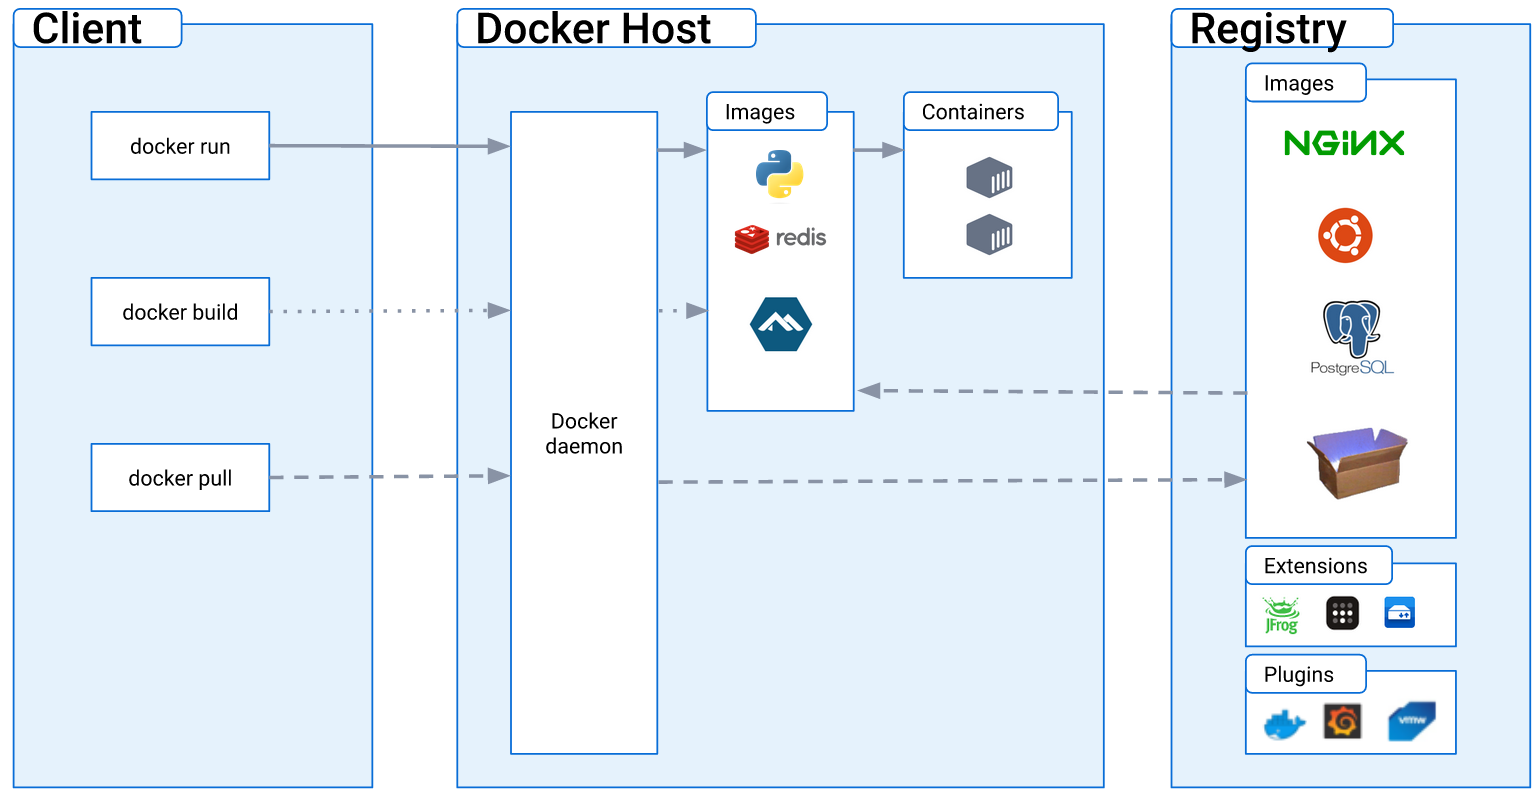
\includegraphics[width=12cm]{figures/docker_architecture.png}
    \caption{Docker Architecture \cite{docker_architecture_ref}.}
    \label{fig:docker_architecture}
\end{figure}

Fig. \ref{fig:docker_architecture} depicts the architecture Docker follows. Several services can be found:

\begin{itemize}
    \item \textit{Docker daemon (dockerd)}, which listens for Docker API requests and deals with managing Docker objects, meaning images, containers, networks, and volumes.
    \item \textit{Docker client}, which is the primary way users interact with Docker. Commands like \texttt{docker run} are sent to \textit{dockerd}, which takes further action on them.
    \item \textit{Docker Registries}, that stores Docker images. Docker Hub is an example of a public registry where Docker looks for images by default.
    \item \textit{Docker Images} is a read-only template with instructions for creating a container. Each of these instructions creates a layer in the image, which is later used when changed and a new image is rebuilt. Only the layer which was modified is rebuilt, which improves the speed of the rebuilding process of containers.
    \item \textit{Docker Containers}, which are runnable instances of images. They can connect to various networks and attached storage. As referred to, a container is no more than a set of layers, and its last layer is always a read-write one, allowing the creation and modification of files and directories in the local filesystem of the container.
\end{itemize}

To conclude, \textit{LXC} (Linux Containers) and \textit{cgroups} (control groups) play a significant role in Docker's underlying architecture. \textit{LXC} is a lightweight operating system-level virtualization method for running multiple isolated Linux systems, known as containers, on a single Linux host. It provides the necessary tools, kernel features, and interfaces to create and manage containers. Each container operates as an independent environment with its own file system, processes, and network stack while sharing the host's kernel. Historically, Docker used \textit{LXC} to create and manage containers by leveraging Linux kernel namespaces and control groups. However, it later replaced it with its own runtime called ``libcontainer''. This change allowed Docker more control over the containerization process and reduced its dependency on external tools.
On the other hand, \textit{cgroups}, a Linux kernel feature that allows the allocation and isolation of system resources among different processes, are extensively used. \textit{Cgroups} provide a mechanism for managing, monitoring, and prioritizing CPU, memory, disk I/O, and other system resources, enabling fine-grained resource allocation and control. Whenever a Docker container is created, a \textit{cgroup} is assigned to it and acts as a resource controller for the container, enforcing limits and restrictions over it. These restrictions involve CPU and memory limits, among others, ensuring containers operate within defined boundaries and efficiently use the host system.

\subsubsection{Ansible} \label{sec:selected_tools_ansible}

Ansible is an open-source automation tool that deals with infrastructure provisioning, configuration management, and application deployment, among other manual processes. Contrary to some of the tools presented in Table \ref{tab:comparison_iac_tools}, Ansible uses a client-only architecture and works by connecting to a machine over standard SSH by default and pushes instructions that could have otherwise been executed manually. These instructions use Ansible modules based on specific endpoint criteria and point to the desired state of the target machine. Ansible does not require additional servers, daemons, or databases, which turns it into quite an interesting tool.

When installing and configuring an application in a server or cloud endpoint, there is a need to perform infrastructure provisioning tasks. When the number of machines to provision is extremely large, it is not feasible to manually issue commands for all of them. Therefore, Ansible creates a set of procedural instruction playbooks in the YAML format that configure a set of managed nodes that make up an Ansible inventory. As with Docker, Ansible is also a tool widely used in the context of CI/CD DevOps pipelines, as entire deployments can be done using a set of playbooks.

As mentioned, SSH is commonly used to connect to managed nodes. Still, other options can be considered, for instance: Kerberos, Lightweight Directory Access Protocol (LDAP), and other centralized authentication management systems. Regarding credential storage, Ansible provides a service that encrypts this information called Ansible Vault.

As for which machines Ansible manages, a simple INI file can be used to make groups of our own choosing. An example of a plain text inventory file looks like this:

\begin{lstlisting}[caption=Ansible Example Inventory file.,numbers=none,label={lst:ansible_inv}]
[webservers]
www1.example.com
10.10.2.3

[dbservers]
db0.example.com
db1.example.com
\end{lstlisting}

Listing \ref{lst:ansible_inv} shows two groups named ``webservers'' and ``dbservers'' respectively, that were created and whose child items can be represented either by a Fully Qualified Domain Name (FQDN) or an IP address. Afterward, variables can be assigned to the group or specific hosts in the inventory file or special directories.

\begin{figure}[H]
    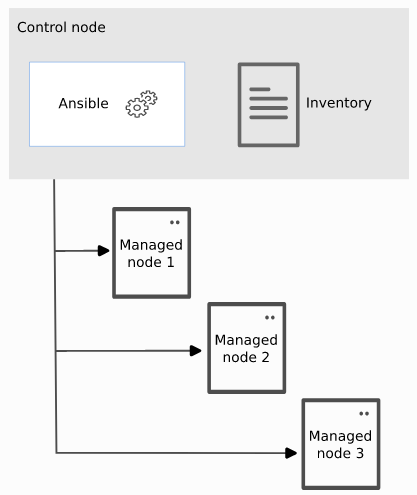
\includegraphics[width=5cm]{figures/ansible_scheme.png}
    \caption{Ansible Schema \cite{ansible_schema_ref}.}
    \label{fig:ansible_schema}
\end{figure}

Fig. \ref{fig:ansible_schema} depicts a general view of how Ansible works, showing the control node, the system on which Ansible is installed, and in which an inventory file composed of a set of managed nodes is placed. These last ones will be later pushed with previously defined configurations.

\subsubsection{Vagrant} \label{sec:selected_tools_vagrant}

Vagrant is another open-source tool that creates a local environment that mimics the environment upon which code will eventually be deployed. It simplifies the creation and management of VMs, simplifying the process of reproducing an environment across different operating systems and platforms.

Several concepts need to be considered when focusing on how Vagrant works. Firstly, we need to consider the existence of a configuration file, the "\textit{Vagrantfile}", which defines the desired state of a VM. This file uses "boxes" as base images for creating VMs, similar to what happened in with Docker. Essentially, a box is a minimal operating system image further customized and provisioned by Vagrant. Moreover, we need to be aware of the concept of "providers", which take care of the creation, management, and execution of VMs. Examples include VirtualBox, VMware, and Hyper-V. Vagrant also supports using Docker as a provider, which allows development environments to be backed by Docker containers rather than VMs. Regarding the provisioning of the VMs, configuration management tools such as Ansible can automatically set up and configure the VMs. Lastly, as with Docker, it allows the creation of synchronized folders between the host machine and the Virtual Machine, and network-related configurations.

\subsubsection{Tailscale} \label{sec:selected_tools_tailscale}

Another selected tool that is worth mentioning is Tailscale which is a mesh VPN service that connects devices and applications in a secure and effortless way. It uses encrypted point-to-point connections using the WireGuard protocol. At first, Tailscale tries to connect devices point-to-point using a coordination server that is used to help nodes find each other by exchanging information on how they should connect, similar to the process of ``Hole Punching'', which is a NAT traversal process to directly connect two devices\footnote{\url{https://en.wikipedia.org/wiki/Hole_punching_(networking)}}. When, for some reason, this is not possible, maybe because the devices are using Symmetric NAT, meaning they only accept connections from peers they've previously connected to, Tailscale uses Designated Encrypted Relay for Packets (DERP) relay servers, and so, traffic remains end-to-end encrypted. This process is called TURN (Traversal Using Relays around NAT).

Conventional VPN services have a "Hub-and-Spoke" where each client device connects to a central VPN gateway. This way, in a Hub-and-Spoke model, if we had a situation in the network where we needed ten fully connected nodes, the central hub would need to have data on nine nodes only, which is more straightforward than having ninety separate tunnel endpoints and know each node's public key, public IP address, and port number. With the Hub-and-Spoke model, we only need to know the static IP address of the central hub to which each node should connect. Some concerns should be addressed if this central hub is far from the remote devices, which can incur high-latency connections. This can be addressed using a multi-hub setup, with hubs/servers distributed across different geographical locations. With this setup, each client device needs a static IP address, an open firewall port, and a set of WireGuard keys. Still, some issues are introduced when, for instance, a new user is added, and there is the need to distribute a new WireGuard key pair to every network device.

A different and more efficient network schema that allows direct communication between nodes, contrary to the Hub-and-Spoke model, is the so-called ``Mesh Networks'' and consists of a set of WireGuard peer-to-peer connections, as presented in Fig. \ref{fig:tailscale_mesh}.

\begin{figure}[H]
    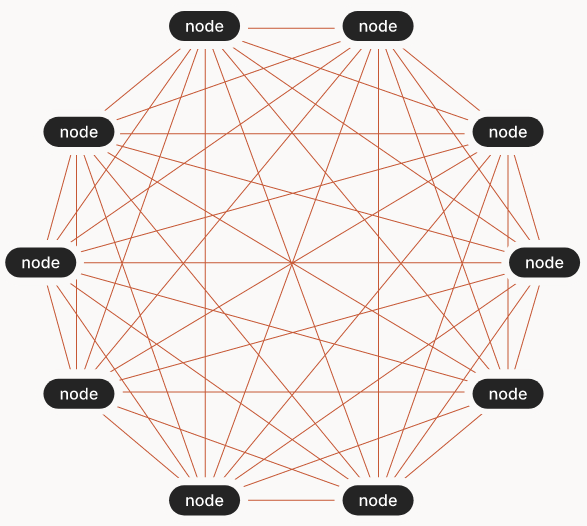
\includegraphics[width=10cm]{figures/tailscale_meshnetwork.png}
    \caption{Point-to-Point Mesh Network \cite{tailscale_docs_ref}.}
    \label{fig:tailscale_mesh}
\end{figure}

Several problems arise from this configuration, like key distribution, node discovery, and firewalls that should allow incoming connections.

For the first problem, Tailscale uses the above-mentioned "coordination server", essentially a shared drop box for public keys. Here we get back to the Hub-and-Spoke model, but Tailscale claims these coordination servers carry virtually no traffic as only a few tiny encryption keys and policies are exchanged. The data plane is a mesh where the actual traffic is located. Typically the steps followed by a new node are as follows:

\begin{itemize}
    \item Every node generates a unique public/private key pair and links the public key to its identity.
    \item The node establishes communication with the coordination server and provides its public key along with information on its current location and domain.
    \item The node downloads a set of public keys and addresses within its domain from the coordination server. Other nodes have previously shared these keys.
    \item The node configures its WireGuard instance by incorporating the relevant set of public keys.
\end{itemize}

Next, the coordination server must know which public keys should be sent to which nodes. This is achieved via authentication, and several options are supported, from 2-Factor Authentication (2FA) or Multi-Factor Authentication (MFA), SMS, Google Authenticator, Gmail, OAuth2, OIDC (OpenID Connect), and SAML providers, among others. With this setup in mind, the authentication process is mostly outsourced because all the account and login data of a specific Tailscale network domain is hosted in another platform. After the authentication process, the public keys of each node are downloaded, and a WireGuard tunnel is configured for each of the network's nodes.

At last, it is essential to mention the NAT traversal feature offered by Tailscale, which turns connection between two nodes sitting behind separate NAT firewalls possible without ever needing to open a firewall port or configure a static IP address. The protocols used by Tailscale to achieve this are STUN (Session Traversal Utilities for NAT) and ICE (Interactive Connectivity Establishment)\footnote{\url{https://tailscale.com/blog/how-nat-traversal-works/}}. Essentially, ICE is a framework that allows peer-to-peer connections. ICE, in turn, uses STUN and/or TURN servers to accomplish this. TURN was mentioned before and was related to relay servers that simply forward packets between two clients. STUN is a protocol that discovers the peers' public addresses and determines restrictions that may prevent a direct connection between them. Notice that no firewall configuration changes are needed as Tailscale, by default, uses HTTPS traffic, for which most firewalls and network setups allow outbound connections. This approach helps to bypass firewall restrictions that may block connections.

\section{Related Work} \label{sec:cyber_ranges}

As explained, cyber ranges are mainly focused on virtualization and containerization. Nonetheless, the research of the current \textit{state-of-the-art} still shows a slight focus on physical hardware.

\subsection{Hardware-based Cyber Ranges} \label{sec:hardware_based_cr}

% National CR

According to Ferguson \textit{et al.} \cite{national_cr_ref}, the National Cyber Range (NCR), closely tied to the American Department of Defense, provides a ``\textit{unique environment for cybersecurity testing throughout the program development life cycle using unique methods to assess resiliency to advanced cyberspace security threats}''. The NCR works as an Internet-like environment supported by a multitude of Virtual Machines and physical hardware. Scenarios are deployed to perform tests that should not occur on open operational networks due to potentially catastrophic consequences caused by the execution of malicious payloads. It features traffic generation techniques, several types of vulnerability scanning, exploitation, and data capturing tools. As expected, the main focus of this project is purely military, meaning there are few details on the internals of the cyber range.

\begin{figure}[H]
    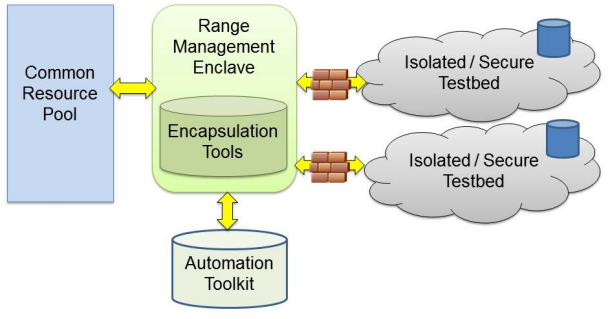
\includegraphics[width=10cm]{figures/ncr_core_capabilities.png}
    \caption{NCR Core Capabilities \cite{national_cr_ref}.}
    \label{fig:ncr_core_capabilities}
\end{figure}

As depicted in Fig. \ref{fig:ncr_core_capabilities}, a firewall is placed between the "Isolated Testbeds" and the "Range Management Enclave". The latter consists of encapsulation tools and an automation tool kit that provisions resources from a "Common Resource Pool". Physical Layer 1 switching ensures isolation concerning the low-level communication protocol stack.  

\begin{figure}[H]
    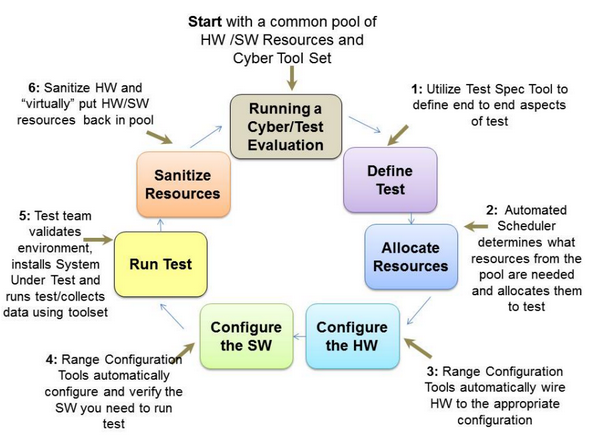
\includegraphics[width=10cm]{figures/ncr_test_evaluation.png}
    \caption{NCR Test and Evaluation Event Execution \cite{national_cr_ref}.}
    \label{fig:ncr_test_evaluation}
\end{figure}

Fig. \ref{fig:ncr_test_evaluation} shows the sequence of actions required to execute tests. Firstly, testing starts with assigning hardware and software resources from the "Common Resource Pool". Afterward, the provisioning process includes using the Layer 1 switch to isolate the selected resources from all the other NCR assets. At this point, the systems under test are installed, and the final network state is matched against the initial expectations. Then, tests are performed, and results are collected. Lastly, hardware is sanitized, ensuring no remnants related to the test, and it is made available back in the "Common Resource Pool".

Gustafsson \textit{et al.} \cite{crate_ref} proposes CRATE, a cyber range heavily relying on a dedicated hardware platform, and the topic of Section \ref{sec:vm_cr}, virtualization.

\begin{figure}[ht]
    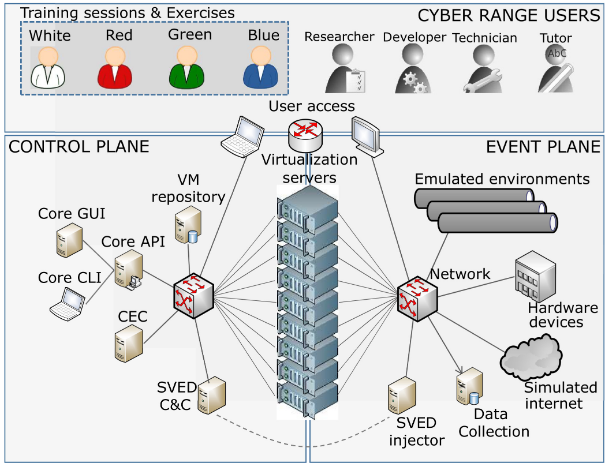
\includegraphics[width=10cm]{figures/crate_architecture.png}
    \caption{CRATE Architecture \cite{crate_ref}.}
    \label{fig:crate_architecture}
\end{figure}

Fig. \ref{fig:crate_architecture} shows a high-level architecture of this system. It is featured with a set of \textit{virtualization servers} that house the emulated environments, a \textit{control plane} used for management tasks, and the \textit{event plane} for systems where training sessions are executed. Inside each virtualization server, a customized Linux-based operating system called CrateOS was placed. Among many other features, it contains a system service named NodeAgent that handles communication between the Core API, which connects to the Application Layer, the Database layer, and the VMs. It automates the deployment and configuration activities of the cyber range. The network in the event plane uses Software Defined Networking (SDN) to facilitate automated configuration and emulation of the networks. Besides, virtual network segments, VXLANs, are used to support many emulated networks. Furthermore, CRATE \textit{Exercise Control (CEC)} is a tool used to set up and manage training sessions. \textit{SVED (Scanning, Vulnerabilities, Exploits, and Detection)} is used to automate experiments and training scenarios. It consists of several modules: one linked to vulnerability data and automatic scans performed with OpenVAS\footnote{\url{https://www.openvas.org/}}, and others related to designing attack graphs, executing them, and generating reports. CRATE allows connecting any hardware device in the emulated environments to conduct experiments with hardware-based security solutions. It is featured with traffic generation tools and data collection tools, using \textit{tcpdump}\footnote{\url{https://www.tcpdump.org/}} and \textit{Snort}\footnote{\url{https://www.snort.org/}}.

\subsection{VM-based Cyber Ranges} \label{sec:vm_cr}

% CyRIS & CyTrONE

Most current \textit{state-of-the-art} focuses on cyber ranges based on Virtual Machines. Pham \textit{et al.} \cite{cyris_ref} proposes a system, CyRIS (Cyber Range Instantiation)\footnote{\url{https://github.com/crond-jaist/cyris}}, that automatically prepares and manages cyber ranges for cybersecurity training based on custom specifications. CyRIS is part of CyTrONE\footnote{\url{https://github.com/crond-jaist/cytrone}} \cite{cytrone_ref}, a training framework that facilitates training activities providing an open-source set of tools that automate the training content generation. It also integrates with a Learning Management System, Moodle. 

\begin{figure}[ht]
    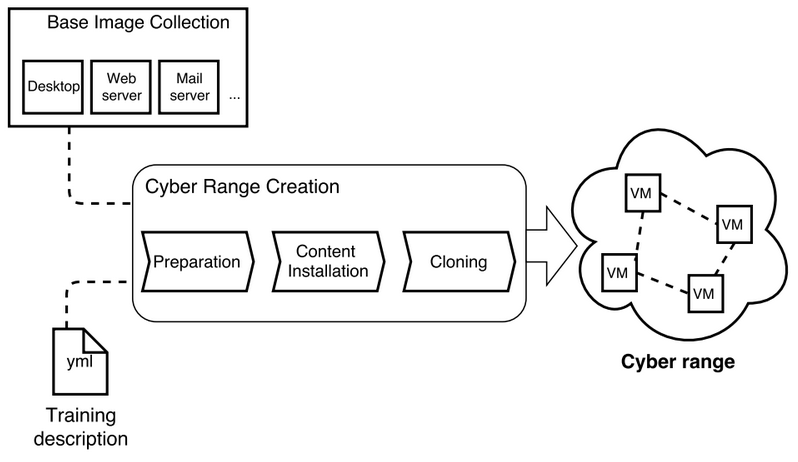
\includegraphics[width=9cm]{figures/cyris_workflow.png}
    \caption{CyRIS Working Flow \cite{cyris_ref}.}
    \label{fig:cyris_workflow}
\end{figure}

According to Fig. \ref{fig:cyris_workflow}, CyRIS is a module that takes a configuration input file following the YAML format and a base image under the format used for KVM virtualization, creating the desired environment according to the provided description. This base image contains a set of pre-installed operating systems and several basic system configurations (hostname, SSH keys, IP addresses). Later on, a master node running the CyRIS service processes the description file and allocates VMs that will be assigned to other hosts of the same LAN network, as observed in Fig. \ref{fig:cyris_architecture}.

\begin{figure}[H]
    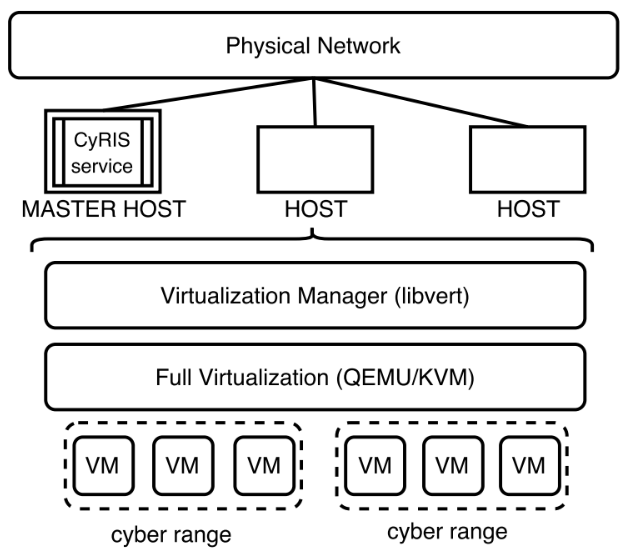
\includegraphics[width=7cm]{figures/cyris_architecture.png}
    \caption{CyRIS's Architecture \cite{cyris_ref}.}
    \label{fig:cyris_architecture}
\end{figure}

CyRIS comprises five key features that play important roles in its architecture:

\begin{itemize}
    \item \textit{System Configuration}, which not only involves basic system configuration but also managing user accounts and modifying firewall rules.
    \item \textit{Tool Installation}, which is essential for the penetration testing work.
    \item \textit{Incident Emulation}, as per the ability to launch actual incidents. It consists of attack emulation, traffic capture, and malware emulation.
    \item \textit{Content Management} consisting of copying content into the cyber range, executing scripts, and generating logs.
    \item \textit{Clone Management}, which considers the defined network topology for the VMs and the inherent isolation between them.
\end{itemize}

Beuran \textit{et al.} \cite{cytrone_ref} presents CyTrONE that follows the architecture presented in Fig. \ref{fig:cytrone_architecture}, where CyRIS is also represented.

\begin{figure}[H]
    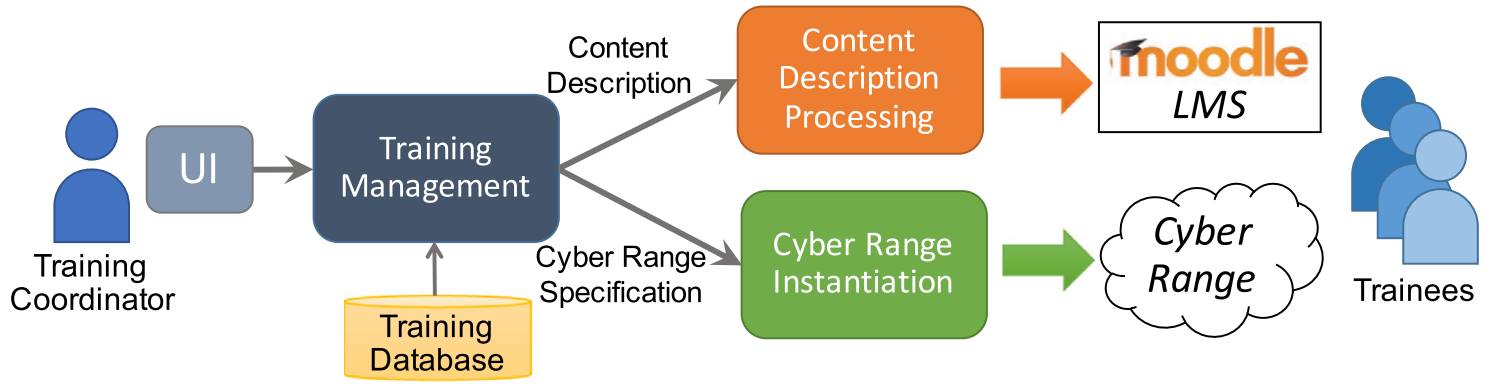
\includegraphics[width=10cm]{figures/cytrone_architecture.png}
    \caption{CyTrONE's Architecture \cite{cytrone_ref}.}
    \label{fig:cytrone_architecture}
\end{figure}

The \textit{Training Management} module is based on user inputs and the training database, which includes training scenarios (VM base images), security incidents, and vulnerability information. This module is responsible for creating the input files related to \textit{content description} and a \textit{cyber range description} defining the training's content and activity. The \textit{Content Description Processing} module converts the content description to a format named SCORM, which is widely used in the e-learning industry and, therefore,  understandable by Moodle. The adoption of Moodle is related to educational purposes and follows a Q\&A approach, as questions related to the posed challenge will be presented on this platform.

% SmallWorld

Like CyTrONE, Furfaro \textit{et al.} \cite{cloud_based_platform_ref} proposes another platform, SmallWorld, also integrated with e-learning systems that explores both virtualization and cloud technologies to reproduce a realistic hybrid environment. Here, the concept of autonomous software agents that imitate the behaviors of human users or malicious actors is introduced. The Agents' behavior is defined via an XML \textit{Agent Definition Language} (ADL) that describes a finite state automaton of the agents' states, possible transitions, and actions. This intermediate representation is later translated into executable code. This tool is featured with a Software Development Kit (SDK) that handles interaction with other tools and allows for the development of customized plug-ins. It uses its own customized \textit{Scenario Definition Language} (SDL) to describe the scenario properties, similarly to other projects. As it is common in VM-based scenarios and due to the possibility of deploying this system in the cloud, this system defines a VPN entry point for accessing the scenario from the exterior.

\begin{figure}[H]
    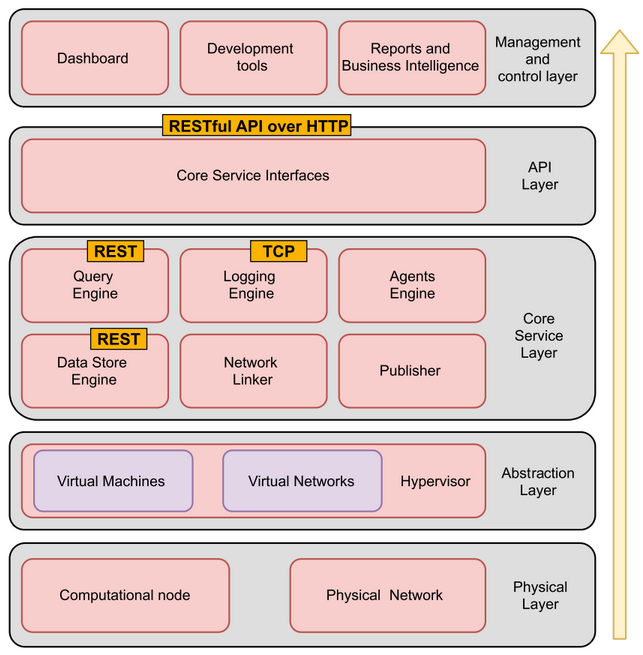
\includegraphics[width=10cm]{figures/smallworld_architecture.png}
    \caption{SmallWorld's Architecture \cite{cloud_based_platform_ref}.}
    \label{fig:smallworld_architecture}
\end{figure}

Fig. \ref{fig:smallworld_architecture} depicts the multi-layered architecture of SmallWorld, which consists of the following:

\begin{itemize}
    \item \textit{Physical Layer}: where computational, storage, and networking hardware is configured to offer fault tolerance and business continuity. It features routers, switches, firewalls, Storage Area Networks (SAN), servers, and other networking services.
    \item \textit{Abstraction Layer}: that relies upon cloud and virtualization technologies, such as OpenStack\footnote{\url{https://www.openstack.org/}}, VirtualBox\footnote{\url{https://www.virtualbox.org/}} or Amazon EC2\footnote{\url{https://aws.amazon.com/ec2/}}, to manage the entire virtual network infrastructure through a hypervisor. 
    \item \textit{Core Service Layer}: where the main software components are hosted. For instance, the "Network Linker" ``\textit{communicates with the underlying network hypervisor and introduces facilities to manage the networking services}'', the "Publisher" ``\textit{is responsible for installing applications (...) and agents in a scenario}'', the "Datastore Engine" ``\textit{handles information that must be stored into suitable databases based on the data type}'' and is later queried by the "Query Engine", the "Agent Engine" that handles the behavior of agents and the "Network Linker" that takes care of statistical data about the running scenario.
    \item \textit{API Layer}: an API connecting to the services below. 
    \item \textit{Management and Control Layer}: where management and development tools rest upon.
\end{itemize}

% Pandora

Jiang \textit{et al.} \cite{pandora_ref} mentions a particularly interesting VM-based type of cyber range, Pandora, which is intentionally incompatible with enterprise systems to reduce the risk of attack propagation into the infrastructure. It proposes a system suitable for automated testing of exploits and result collection, keeping security concerns related to the sandboxed environment in mind by considering vulnerabilities on VMware Fusion (CVE-2015-2337) and Venom (CVE-2015-3456) that allowed VM escape, thereby causing damage to host systems. 

\begin{figure}[H]
    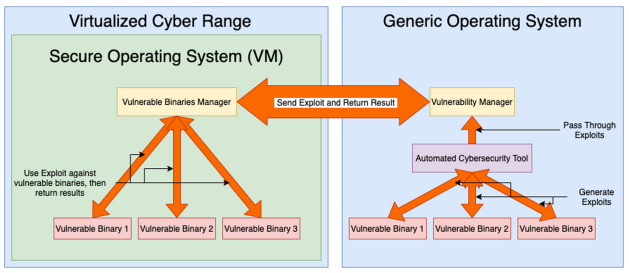
\includegraphics[width=14cm]{figures/pandora_architecture.png}
    \caption{Pandora's Architecture \cite{cytrone_ref}.}
    \label{fig:pandora_architecture}
\end{figure}

Fig. \ref{fig:pandora_architecture} portrays Pandora's architecture, which runs under a VM with an operating system that introduces some incompatibility with the "Generic Operating System" to, as mentioned before, introduce an intentional inconsistency with regards to damage propagation outside the testing environment. The "Vulnerable Binary Manager" is used to execute vulnerable binaries within the secure environment, use exploits against the vulnerable binary and record the effect of such exploitations. A "Vulnerable Binary" is a file containing a set of defined vulnerabilities that automated tools will exploit. Notice that this binary should only be able to be executed within the "Secure OS". The "Vulnerability Manager" is an API that handles communication with the cyber range by sending exploits and receiving responses from the "Vulnerable Binary Manager". The "Automated Cybersecurity Tool(s)" generates exploits against vulnerable binaries and is not present in the secure operating system to assure simplification. Examples include fuzzing tools, such as Fuzzer\footnote{\url{https://github.com/angr/phuzzer}} and American Fuzzy Lop\footnote{\url{https://lcamtuf.coredump.cx/afl/}} to generate crash strings for simple binary files vulnerable to buffer overflows. Later on, rex\footnote{\url{https://github.com/angr/rex}}, an automated exploit engine, exploits the target binary using the above-mentioned crash string obtained from the fuzzing tool, generating a Proof of Vulnerability (POV) that is later on sent to the "Vulnerability Manager" and received by the "Vulnerability Binary Manager" inside the cyber range VM.

More theoretically speaking, Debatty \textit{et al.} \cite{building_cr_ref} stresses the need for cyber ranges to improve Cyber Defense Situation Awareness (CDSA). 

\begin{figure}[H]
    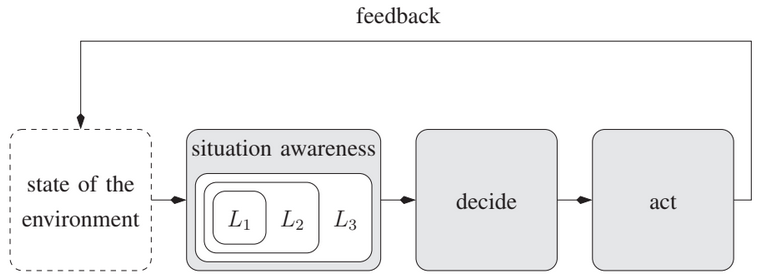
\includegraphics[width=10cm]{figures/building_cr_endsley_model.png}
    \caption{Endsley's Decision Making Model \cite{endsley_ref}.}
    \label{fig:endsley_decision_making_model}
\end{figure}

The speed at which events unfold during a cyber incident requires an efficient decision-making process. Fig. \ref{fig:endsley_decision_making_model} shows Boyd and Endsley \cite{endsley_ref} decision-making model that plays an important role in CDSA. Three levels of \textit{"Situation Awareness"} (SA) are discussed \cite{building_cr_ref}:

\begin{itemize}
    \item \textit{Level 1 SA (\textit{"perception"})}: ``\textit{perceive the real-time status, attributes, and dynamics of relevant elements in cyberspace}''. This entails activities such as monitoring the network and detecting anomalies. This concept is closely tight to the idea of \textit{"Security Operations Centre"} (SOC) and \textit{"Security Incident and Event Management"} (SIEM).
    \item \textit{Level 2 SA (\textit{"comprehension"})}: ``\textit{aggregation and assessment of level 1 information in order to understand how the current situation impacts our goals and objectives}''. This refers to the construction of attack graphs outlining the attack details.
    \item \textit{Level 3 SA (\textit{"projection"})}: ``\textit{the ability to extrapolate the actions of the elements in cyberspace into the future, based on L2 comprehension of the current situation}''.
\end{itemize}

Endsley's model situation awareness is achieved using \textit{"mental models"} which, according to Rouse and Morris \cite{rouse_morris_ref}, are ``\textit{mechanisms whereby humans can generate descriptions of system purpose and form explanations of system functioning and observed system states, and predictions of future states}''. It is precisely this that cyber range training aims to improve.

Following this stream of thought, Debatty \textit{et al.} \cite{building_cr_ref} proposed a VM-based cyber range where YAML/JSON description files are used to define the final state of the deployed scenario. Inside this description file, it is possible to include Ansible playbooks that provide additional software to the scenario. It uses Vagrant images as VMs and allows their customization: the number of vCPUs, amount of memory, number of network interfaces, operating system, and installed software. This enables the creation of VMs that are Intrusion Detection Systems, traffic generators, systems that encompass a set of analysis tools made available for the trainees, or simply a vulnerable server that should be hacked during the challenge. The main components of the cyber range are the hypervisor, a Remote Desktop Gateway, to allow remote desktop access to VMs, either using Remote Desktop Protocol (RDP), Virtual Network Computing (VNC), and an orchestrator node that provisions and instantiates the VMs. Currently, this project uses Apache Guacamole\footnote{\url{https://guacamole.apache.org/}}, which supports both RDP and VNC, to allow users to connect to the cyber range via a browser.

Yamin \textit{et al.} \cite{serious_games_as_a_tool_to_model_attack_and_defense_scenarios_ref} proposes a set of cyber range scenarios based in a game, consisting of attackers wanting to compromise a network and defenders preventing such from happening. A Domain-Specific Language (DSL) defines each scenario's main properties, allowing for specific customization, similar to previous projects. The abstract syntax of DSL targets scenario properties, the internal configuration of VMs, routing configurations across the virtualized environment, services, vulnerabilities within VMs, agent tasks related to traffic generation, autonomous attack launching, and others. A concrete syntax in YAML, derived from DSL, is used to create the final instances of the scenario. After validation and compilation of this syntax, a set of HEAT templates are generated and used by OpenStack to deploy a Virtual Machine network in a private cloud. For the configuration and provisioning of VMs, Ansible is used.

% Leaf

Ficco \textit{et al.} \cite{leaf_ref} mentions a complex cyber range especially tailored for Internet Of Things (IoT) scenarios and Edge applications. Apart from the standard features of these types of cyber ranges, it includes a gorgeous user interface and a complex monitoring system where events are collected via firewalls, IDS, and due to network traffic analysis. Events also refer to machine monitoring operations, for instance, if a machine is not responding or a particular port is open or closed. These sorts of events should be communicated to those outside the cyber range, meaning an API must be made available. This project was developed using technologies like pfSense, an open-source software that emulates firewalls, routers, DHCP servers, DNS servers, and VPN endpoints. Three virtualization technologies were tested: VMware ESXi, OpenStack, and Oracle VirtualBox. VMware ESXi and OpenStack are used for remote deployments. VirtualBox is for smaller local deployments, meaning cyber range VMs are distributed as OVA files. Details on network configuration with pfSense, firewall rules, management of Certification Authorities (CA) and SSL certificates for encrypted traffic between servers and users that go through pfSense, creation of groups within the network with several layers of privileges, references to OpenVPN, which comes installed by default installed in pfSense, Network Address Translation (NAT) and DNS configurations are highly detailed in this article.

Bernardinetti \textit{et al.} \cite{nautilus_ref} cites Nautilus, a VM-based cyber range that leverages cloud technologies to semi-automate the deployment of vulnerable virtualized networks. It includes a platform-agnostic configuration language for the scenarios aiming for local and remote deployments. Additionally, it uses Vagrant and Ansible for software provisioning. Essentially, Nautilus works on top of any hypervisor, such as VirtualBox, VMWare, KVM, and Amazon AWS, among others. Configuration files for the VMs are written in a \textit{Vagrantfile}, including hardware specifications, the base image to use, and network configurations. A set of Ansible playbooks describe how to provision the VM. All this is done using Nautilus SDL, meaning these high-level descriptions of the scenes are parsed, and the outcome serves as input for Ansible and Vagrant.

Lastly, Russo \textit{et al.} \cite{crack_ref} suggests CRACK, a cyber range that uses an SDL for declaring scenarios and supports automatic verification of the training objects of the scenario. The SDL can be translated into Datalogs as part of declarative programming logic, which are later used for executing test cases on the scenario. It follows an approach interrelated to IaC for cloud deployment of Virtual Machines. 

\subsection{Container-based Cyber Ranges}

Container-based cyber ranges are frequently linked to reduced resource consumption compared to VM-based scenarios, mainly because the container's resources are shared with the host, causing a lower overhead. This same overhead is even lower compared to scenarios full of virtual instances since the CPU and memory usage compared to VM-based scenarios is much lower. According to Thompson \textit{et al.} \cite{labtainers_ref}, Docker containers have several advantages:

\begin{itemize}
    \item \textit{File system isolation}: each container runs in a separate root file system.
    \item \textit{Resource isolation}: system resources such as CPU, network bandwidth, and memory are allocated according to the process container using \textit{cgroups}, for instance. This is important considering several labs running within the same host machine, where unfair resource allocations should be prevented.
    \item \textit{Network isolation}: each container runs within its network namespace consisting of a virtual interface and specific IP address.
    \item \textit{Copy-on-write}: containers' file systems are created using copy-on-write (COW), an optimization strategy when multiple callers ask for resources. Initially, they are given pointers to the same resource. However, if a modification is needed, a private copy of the resource is created to prevent changes from being visible to every caller. This ensures fast deployments, cheap in terms of memory and disk.
    \item \textit{Change management}: changes to a container's file system result in a new image that other containers can reuse.
    \item \textit{Interactive shell}: there is the possibility of allocating a pseudo-tty and attaching the standard input of any container, essentially translated to the fact that a prompt can be obtained to access the internals of the container.
\end{itemize}

This section intends to elaborate on container-based cyber ranges and their specific details.

% DSP

Perrone \textit{et al.} \cite{dsp_ref} brings forward the \textit{Docker Security Playground}\footnote{\url{https://github.com/DockerSecurityPlayground/DSP}}, a microservices-based approach to build complex network infrastructures tailored to study network security. These microservices are based on Docker. Likewise, it offers an API enabling further development on the lab scenarios. This project uses Docker-compose to manage scenarios' start and stop procedures. It uses a \textit{Docker Image Wrapper} which defines a standard notation for Docker labels to provide custom configurations for the base Docker image of each scenario. The Docker images used within the project are placed at DockerRegistry Hub\footnote{\url{https://hub.docker.com/u/dockersecplayground}}.

% Capturing flags in a dynamically deployed microservices-based heterogeneous environment

Related to the \textit{Docker Security Playground}, Caturano \textit{et al.} \cite{capturing_flags_ref} designed another container-based cyber range built upon the \textit{Docker Security Playground}. This project tackles the fact that several vulnerabilities related to the kernel cannot be explored in Docker-based environments because containers share the Linux kernel with the Docker host. To overcome this problem, Capturano \textit{et al.} explores scenarios based on containers and Virtual Machines, providing a hybrid environment where cybersecurity exercises are deployed. For this, it makes use of \textit{"macvlan"} interface drivers to create a bridge between Docker containers and VMs. Similarly, Acheampong \textit{et al.} \cite{security_scenarios_automation_ref} mixes the concept of cloud deployments based on Virtual Machines with Docker containers hosting packaged applications.

Closely related to the education side, Thompson \textit{et al.} \cite{labtainers_ref} refers to another training framework, Labtainers\footnote{\url{https://github.com/mfthomps/Labtainers}}, which relies on Docker containers featured with an automatic assessment of students, as lab data is collected and automatically sent to an instructor upon completion via email or an LMS, creating the possibility of analyzing the experiential learning efficacy of the exercise. Specific properties of the laboratory activities are randomized so that each student works on a different scenario in terms of configurations. This randomization is achieved by defining symbols within the source code and data files part of the lab, which are replaced with student-specific values upon lab startup, for instance, the buffer size related to a buffer overflow vulnerability. This concept is further explored in the next section.

\subsection{Randomization} \label{sec:randomization_cr}

Developing a scenario for a cyber range is mainly a manual process. An example that corroborates this statement is SEED Labs \cite{seed_labs_ref}, where many of Labtainers' laboratories are based \cite{labtainers_ref}, where several scenarios based on software security, web security, system security, mobile security, network security, cryptography, and blockchain are made available to trainees using both Virtual Machines and containers. More than 80 universities use SEED Labs, which expresses close bounds to education.

Consequently, there is a need to address some randomization of the developed scenarios as they essentially turn out to be static once created. As so, this section elaborates more on the cyber ranges, both VM-based and container-based, that take into account randomization.

% SecGen

We start with Schreuders \textit{et al.} \cite{secgen_ref} that proposes a VM-based cyber range, SecGen\footnote{\url{https://github.com/cliffe/SecGen}}, developed in Ruby that introduces randomization. It is suited for both educational lab usage and CTF challenges. One of the main concerns is addressing the sluggish pace associated with the manual configuration of hacking scenarios, which is not practical at scale. This cyber range focuses on a CTF-style type of challenge, where solving the proposed challenge results in discovering a secret flag. The introduced randomization is characterized as follows:

\begin{itemize}
    \item \textit{Selection}: randomized selection of the operating system, network configurations, services, system configurations, and vulnerabilities to be used.
    \item \textit{Parameterisation}: that entails system elements should be configurable, for instance, the strength of a user account password.
    \item \textit{Nesting}: data generation should be combined/nested randomly.
\end{itemize}

The description of the system greatly depends on the XML specification language, which states the details related to the configuration of the network, available vulnerabilities, services, users, and content and applies logic for randomizing the scenario. It uses Puppet and Vagrant to provision the VMs. A critical takeaway idea of this project is its highly modular structure and the use of vulnerabilities and associated exploits provided by the Metasploit Framework. The SecGen running process is composed of two stages:

\begin{itemize}
    \item \textit{First Stage}: is where all the scenario Ruby modules are read, randomization steps are applied, and the Puppet modules are deployed. At last, a Vagrant file is created, which describes the entire scene, according to the steps mentioned.
    \item \textit{Second Stage}: leverages Vagrant to generate and provision the VMs. 
\end{itemize}

Currently, SecGen counts over 100 modules: data generation modules, encoder modules, providing various encryption and encoding methods, service modules, providing a wide range of secure services, utility modules, allowing various system configurations, and vulnerability modules, concerning vulnerable services. 

% CyExec

Consequently, Nakata \textit{et al.} \cite{cyexec_ref} proposes a Directed Acyclic Graph (DAG) based cyber range, CyExec, with randomization techniques in mind, using Docker containers. This article claims CyExec outperforms the SecGen VM-based scenario \cite{secgen_ref} generator, consuming 1/3 memory, having 1/4 CPU load, and 1/10 of storage usage, primarily since it uses containers instead of VMs.

The concept of randomization here takes the form of a graph such as the one presented in Fig. \ref{fig:cyexec_randomization}, being each milestone a vertex and each scenario an edge, meaning an attack consists of different types of vulnerabilities that achieve the same outcome. As a result, the trainee experiences several distinct situations. Since the attack is directed towards the final target and there is no going back to a previous milestone or looping back to the same vertex, this graph is considered a DAG.

\begin{figure}[H]
    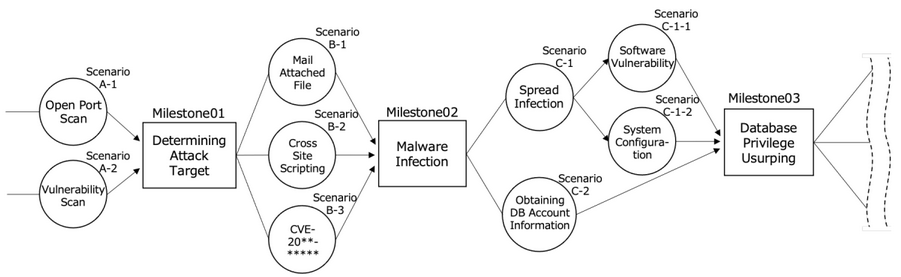
\includegraphics[width=10cm]{figures/cyexec_randomization.png}
    \caption{CyExec randomization \cite{cyexec_ref}.}
    \label{fig:cyexec_randomization}
\end{figure}

Fig. \ref{fig:cyexec_structure} shows the structure followed by CyExec. With several Docker-compose files, randomization is assured because it allows switching between which \textit{Dockerfiles} are used when setting up a scenario. A \textit{Dockerfile} works as just another "edge"  to reach a "vertex", leading us to the fact that different vulnerabilities are introduced into the system according to the selected \textit{Dockerfile}.

\begin{figure}[H]
    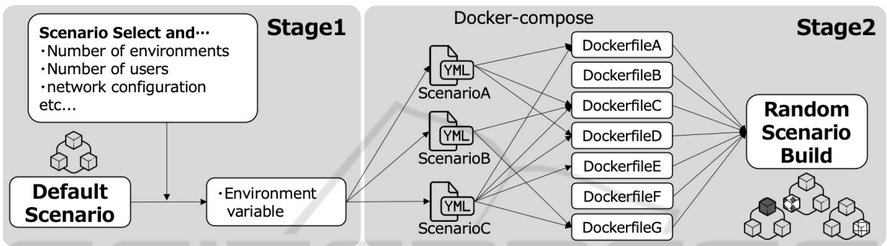
\includegraphics[width=10cm]{figures/cyexec_structure.png}
    \caption{CyExec structure \cite{cyexec_ref}.}
    \label{fig:cyexec_structure}
\end{figure}

For example, consider a scenario where Metasploitable2\footnote{\url{https://docs.rapid7.com/metasploit/metasploitable-2-exploitability-guide/}}, a purposely vulnerable system, is available in the CyExec testbed. Several vulnerable applications can be found in this machine, such as vsftpd, PHP, Samba, and PostgreSQL, among others. Scenarios can be swapped and selected randomly if different vulnerabilities or attack techniques are considered.

% Cloud-based 

\subsection{Threats and Vulnerabilities} \label{sec:threats_vulnerabilities_cr}

When dealing with cyber ranges, it is crucial to consider potential threats and vulnerabilities these systems can introduce, especially when dealing with VM escaping situations \cite{pandora_ref}. As such, Noponen \textit{et al.} \cite{cybersecurity_threat_and_mitigations_ref} deems cloud security issues as relevant because cyber ranges are often located in a cloud. This situation is even more worrisome if we consider private clouds. Besides, it points out that DoS attacks can severely disturb these cyber exercises.

% Threats and Vulnerabilities 

Taib \textit{et al.} \cite{threats_and_vulnerabilities_ref} calls our attention to threats and vulnerabilities existing in dual-stack cyber ranges, where devices can run both IPv4 and IPv6 in parallel. This article performs tests in a VM-based scenario that also makes use of Graphic Network Simulator 3 (GNS3)\footnote{\url{https://gns3.com/}}, a network software emulator. It demonstrates how to enforce constraints on the system via Access Control Lists (ACLs) and host-based firewall rules.

Noponen \textit{et al.} \cite{cybersecurity_threat_and_mitigations_ref} organizes possible threats against cyber ranges according to the following types:

\begin{itemize}
    \item \textit{Physical Threats} that concern local deployments, as devices may be compromised or damaged.
    \item \textit{Communication Threats}, mainly relevant to remotely connected users where an attacker can intercept the traffic associated with the cyber range. Encryption is deemed essential in these types of situations.
    \item \textit{Virtual Machines and Containers}, although likely uncommon, it is essential to consider the possibility of an attacker leaving the sandboxed environment and giving it access to the host machine. MITRE \cite{mitre_containers_issues_ref} introduces an ATT\&CK Matrix for container systems, pointing out privilege escalation issues related to incorrect container privileges and misconfigured bind mounts, among others. Such mistakes may end up allowing malicious access to the underlying system hosting the cyber range.
    \item \textit{Cloud Threats}, which are also referenced by MITRE \cite{mitre_cloud_issues_ref}, similarly to what happened with containers. MITRE also references mitigations against adversary techniques, most related to software updates, deployment of Intrusion Detection and Prevention Systems, policy enforcement, and network segmentation.
\end{itemize}

Regarding cloud security issues, Torkura \textit{et al.} \cite{continuous_auditing_and_threat_detection_ref} proposes a system tested with AWS and Google Cloud that continuously monitors the cloud infrastructure to detect malicious activities, misconfigurations, and unauthorized changes. It includes proactive risk analysis where Common Vulnerability Scoring System (CVSS)\footnote{\url{https://nvd.nist.gov/vuln-metrics/cvss}} is used to score vulnerabilities in the cloud infrastructure, according to their impact and exploitability metrics. Although not used within the context of cyber ranges, this is an example of a project that can be applied to the underlying infrastructure of cyber ranges as a way to perceive if malicious actions are being directed towards the exercise itself.

\section{Summary} \label{sec:summary}

This chapter performed a literature review focusing on the main areas this work aims to build upon: cyber ranges and Infrastructure as Code. 

Starting from the methodology used during the research process, exploring general definitions and concepts related to cyber ranges, and detailing the key features of the gathered references. Hardware-based, VM-based, and container-based cyber ranges were deeply analyzed in order to understand in great detail what the current \textit{state-of-the-art} lacks and perceive, for instance, the necessities of an enterprise-level network, the tools used in attack-based cyber range scenarios, network services exposed, technologies used, among others. Randomization and threats and vulnerabilities exposed by such types of cyber range systems were also addressed, which attackers may leverage using privilege escalation techniques, compromising the existing physical infrastructure supporting the system. 

As mentioned throughout this chapter, current cyber range problems are related to high-cost infrastructure relying too much on Virtual Machines, and details of these kinds of open-source scenarios rarely reference up-to-date vulnerabilities and attacks. Container-based solutions are starting to appear, but they heavily rely on custom cyber range description files, using the YAML, XML, or, sometimes, even the JSON format. There are cases where IaC tools are not being used, hampering scalability concerns. In such cases, a custom tool was typically designed to parse and take action on the aforementioned customized scenario description files. Randomization is clearly lacking in some cyber range scenarios, which is understandable given that developing these testing environments is a slow manual process.

Nonetheless, key takeaway ideas in the performed search are mostly related to the services in the cyber range scenarios, which simulate enterprise-level networks and the technologies used to build them. Other topics that stand out during our search concern traffic generation using automated scripts that emulate benevolent or malicious behavior, and aspects related to monitoring trainee actions across the testing environment are also essential factors that can make the scenario more realistic. Lastly, the set of vulnerabilities and attacks instigated across all references, especially in open-source projects, were very useful for our project's sake to better understand typical scenario examples.

Table \ref{tab:comparison_cr} presents a high-level overview of the main features supported by some of the most relevant cyber ranges, finishing with the proposed solution's aim.

\begin{table}[H]
  \caption{Comparison of Cyber Ranges.}
\scalebox{0.54}{
\begin{tabular}{ | c | c | c | c | c | c | c | c | c |}
\hline
\empty & \textbf{IaC} & \textbf{Randomization} & \textbf{Local \& Cloud Deployments} & \textbf{Containerization} & \textbf{Enterprise-level Scenarios} & \textbf{Linux \& Windows Scenarios} & \textbf{Open-source} \\ 
\hline
\textit{CyExec} & \priority{50} & \priority{100} & \priority{100} & \priority{100} & \priority{50} & \priority{50} & \priority{0} \\  
\hline
\textit{Pandora} & \priority{0} & \priority{100} & \priority{50} & \priority{0} & \priority{0} & \priority{50} & \priority{0} \\
\hline
\textit{CyRIS/CyTrONE} & \priority{50} & \priority{100} & \priority{100} & \priority{0} & \priority{0} & \priority{50} & \priority{100} \\
\hline
\textit{NCR} & - & \priority{100} & \priority{50} & \priority{0} & \priority{0} & - & \priority{0} \\
\hline
\textit{SmallWorld}  & \priority{50} & \priority{0} & \priority{100} & \priority{0} & \priority{100} & \priority{100} & \priority{0} \\
\hline
\textit{Leaf}  & \priority{100} & \priority{100} & \priority{100} & \priority{0} & \priority{100} & \priority{0} & \priority{0} \\
\hline
\textit{CRACK} & \priority{50} & \priority{100} & \priority{50} & \priority{0} & \priority{100} & \priority{50} & \priority{100} \\
\hline
\textit{SEED Labs} & \priority{50} & \priority{0} & \priority{50} & \priority{50} & \priority{50} & \priority{50} & \priority{100} \\
\hline
\textit{Labtainers} & \priority{50} & \priority{100} & \priority{100} & \priority{50} & \priority{100} & \priority{50} & \priority{100} \\
\hline
\textit{CRATE} & - & \priority{100} & \priority{50} & \priority{0} & \priority{100} & \priority{50} & \priority{0} \\
\hline
\textit{DSP} & \priority{50} & \priority{0} & \priority{50} & \priority{100} & \priority{100} & \priority{50} & \priority{100} \\
\hline
\textit{SecGen} & \priority{100} & \priority{100} & \priority{50} & \priority{0} & \priority{100} & \priority{50} & \priority{100} \\
\hline
\textit{\textbf{\specialcell{Proposed\\Solution}}} & \priority{100} & \priority{100} & \priority{100} & \priority{100} & \priority{100} & \priority{100} & \priority{100} \\
\hline
\end{tabular}}
  \label{tab:comparison_cr}
\end{table}

Several marks were given according to each cyber range. As a way to demystify some classifications, for the \textit{IaC} column, we considered half a circle as approaches that used customized descriptions to deploy scenarios or solutions only relying on Docker or Docker-compose without a standard tool, as some of the ones presented in Table \ref{tab:comparison_iac_tools}; for the \textit{Randomization} column, we considered tools that provided some randomization of: traffic generation, network, system, and accounts' configurations or of the vulnerabilities present in the scenario as of a full circle. Regarding the \textit{Local \& Cloud Deployments} and \textit{Linux \& Windows Scenarios}, we considered half a circle for cases where only one of the features was present. About the \textit{Containerization} column, we considered half a circle for scenarios that combined containers and VMs in separate scenarios. Concerning the \textit{Enterprise-level Scenarios} column, we considered full circles as a network with a wide variety of services ranging from firewalls, internal networks, IDS, and mail servers, among others. At the same time, half-circles were intermediate representations of enterprise-level networks. Finally, the \textit{Open-source} column considers scenarios available to the general public.

Our framework addresses every column of Table \ref{tab:comparison_cr}, which is not achieved by any other framework. Even in cyber range frameworks such as \textit{CyExec}, which is complete in terms of the mentioned features, a possible idea would be to extend the development. Unfortunately, not all frameworks are open-source, and some lack community support. Instead, we opted to create a new framework with the functionalities we wanted, using the technology stack of our choice. With this idea in mind, Chapter \ref{chap:problem_statement} will further detail the problem to be solved.